\documentclass{article}
\usepackage{amsmath}
\usepackage{amsfonts}
\usepackage{sectsty}
\usepackage{hyperref}
\usepackage{fancyhdr}
%TODO: FIX MARGINS
\usepackage[top=1in,bottom=1in,left=1in,right=1in]{geometry}
\usepackage{float}
\usepackage{graphicx}
\usepackage{tabularx}

\title{Lecture 1 - Introduction}
\author{Matthew Farah, \href{mailto:farahm11@mcmaster.ca}{$\langle$farahm11@mcmaster.ca$\rangle$}, 400468251}
\date{\today}

\fancyhead{}
\fancyhead[L]{Matthew Farah, \href{mailto:farahm11@mcmaster.ca}{$\langle$farahm11@mcmaster.ca$\rangle$}, 400468251}
\fancyhead[R]{Lecture 1 - Introduction}

\renewcommand{\thesubsection}{\thesection.\alph{subsection}}
\renewcommand{\thesubsubsection}{\thesection.\alph{subsection}.\Roman{subsubsection}}
\makeatletter

\newcolumntype{Y}{>{\centering\arraybackslash}X}
\renewcommand{\arraystretch}{1.8}

\sectionfont{\fontsize{12}{12}\bfseries}
\subsectionfont{\fontsize{10}{12}\normalfont}
\subsubsectionfont{\fontsize{10}{12}\normalfont}

\begin{document}
\maketitle

\begin{itemize}
	\item The study of signals and system concerns itself with the synthesis and interpretation of signals.
	\item Digital signals are discretized.
	\begin{itemize}
		\item Sampling frequencies are used to make discrete signals continuous.
	\end{itemize}
	\item Systems can be described as functions with a memory (capable of remembering past inputs and outputs).
	\begin{itemize}
		\item The output of a system depends on its previous state.
		\item Bears conceptual similarity to state machines.
		\item The input signal to discrete time systems need not be discrete.
	\end{itemize}
	\item The input to and output from a system is typically denoted as $x$ and $y$ respectively.
	\begin{itemize}
		\item Discrete systems use $n$ as their independent variable.
		\begin{itemize}
			\item $n \in \mathbb{N}$.
			\item All inputs and outputs for $n < 0$ are defined to be zero.
			\item NOTE: n does NOT represent time, it represents the current sample or cycle the system is on.
		\end{itemize}
	\end{itemize}
	\item We can represent the inputs and outputs of a discrete system at a given cycle $n$ with a table.
\end{itemize}

At a high-level, we can describe systems with the following diagram:

\begin{figure}[H]
	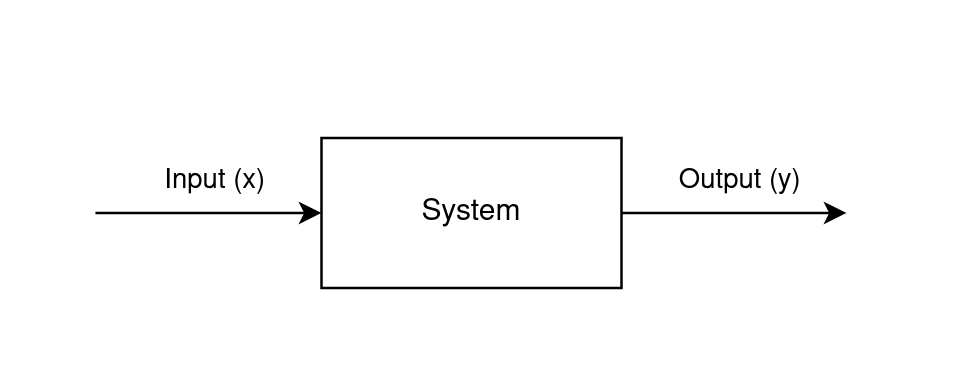
\includegraphics[width=\linewidth]{./imgs/System-Diagram.png}
	\caption{Graphical representation of a system}
	\label{fig:System-Representation}
\end{figure}

\section[Example ~\thesection]{Ex. Compute the outputs to the system $y(n) = \frac{1}{2}x(n) + \frac{1}{2}x(n-1)$ for the following inputs}

Note: This system $y(n) = \frac{1}{2}x(n) + \frac{1}{2}x(n-1)$ has a special name, the ``Truepoint Moving Average''

\subsection[~\thesubsection]{$x(n) = \begin{cases} 1, \; \text{if} \; n = 1, 2, 3 \\ 0, \; \text{otherwise} \end{cases}$}

\begin{tabularx}{\linewidth}{| c || Y Y Y Y Y Y |}
	\hline
	$n$ & 0 & 1 & 2 & 3 & 4 & 5\\
	\hline
	$x(n)$ & 0 & 1 & 1 & 1 & 0 & 0\\
	$y(n)$ & 0 & $\tfrac{1}{2}$ & $\tfrac{1}{2}$ & 1 & $\tfrac{1}{2}$ & 0\\
	\hline
\end{tabularx}


\subsection[~\thesubsection]{$x(n) = \begin{cases} 1, \; \text{if} \; n = 0 \\ 0, \; \text{otherwise} \end{cases}$}

\begin{tabularx}{\linewidth}{| c || Y Y Y Y Y Y |}
	\hline
	$n$ & 0 & 1 & 2 & 3 & 4 & 5\\
	\hline
	$x(n)$ & 1 & 0 & 0 & 0 & 0 & 0\\
	$y(n)$ & $\tfrac{1}{2}$ & $\tfrac{1}{2}$ & 0 & 0 & 0 & 0\\
	\hline
\end{tabularx}

\subsection[~\thesubsection]{$x(n) = \cos(n\pi)$}

\begin{tabularx}{\linewidth}{| c || Y Y Y Y Y Y |}
	\hline
	$n$ & 0 & 1 & 2 & 3 & 4 & 5\\
	\hline
	$x(n)$ & 1 & -1 & 1 & -1 & 1 & -1\\
	$y(n)$ & $\tfrac{1}{2}$ & 0 & 0 & 0 & 0 & 0\\
	\hline
\end{tabularx}

\section[Example ~\thesection]{Ex. Compute the outputs to the system $y(n) = x(n) - y(n-2)$ for the following inputs:} 

\subsection[~\thesubsection]{$x(n) = \begin{cases} 1, \; \text{if} \; n = 0 \\ 0, \; \text{otherwise} \end{cases}$}

\begin{tabularx}{\linewidth}{| c || Y Y Y Y Y Y |}
	\hline
	$n$ & 0 & 1 & 2 & 3 & 4 & 5 \\
	\hline
	$x(n)$ & 1 & 0 & 0 & 0 & 0 & 0 \\
	$y(n)$ & 1 & 0 & -1 & 0 & 1 & 0 \\
	\hline
\end{tabularx}

\subsection[~\thesubsection]{$x(n) = \cos(\frac{1}{2}{\pi}n)$}

\begin{tabularx}{\linewidth}{| c || Y Y Y Y Y Y |}
	\hline
	$n$ & 0 & 1 & 2 & 3 & 4 & 5 \\
	\hline
	$x(n)$ & 1 & 0 & -1 & 0 & 0 & 1 \\
	$y(n)$ & 1 & 0 & -2 & 0 & 3 & 0 \\
	\hline
\end{tabularx}

\section[Example ~\thesection]{Ex. Compute the outputs to the system $y(n) = x(n) +\frac{1}{2}y(n-1)$ where $x(n) = \begin{cases} 1, \; \text{if} \; n = 0 \\ 0, \; \text{otherwise} \end{cases}$}

\begin{tabularx}{\linewidth}{| c || Y Y Y Y Y Y |}
	\hline
	$n$ & 0 & 1 & 2 & 3 & 4 & 5 \\
	\hline
	$x(n)$ & 1 & 0 & 0 & 0 & 0 & 0 \\
	$y(n)$ & 1 & $\tfrac{1}{2}$ & $\tfrac{1}{4}$ & $\tfrac{1}{8}$ & $\tfrac{1}{16}$ & $\tfrac{1}{32}$ \\
	\hline
\end{tabularx}

\section[Example ~\thesection]{Ex. Compute the outputs to the system $y(n) = x(n) + x(n-1) - y(n-1)$ where $x(n) = n + 1$}

\begin{tabularx}{\linewidth}{| c || Y Y Y Y Y Y |}
	\hline
	$n$ & 0 & 1 & 2 & 3 & 4 & 5 \\
	\hline
	$x(n)$ & 1 & 2 & 3 & 4 & 5 & 6 \\
	$y(n)$ & 1 & 2 & 3 & 4 & 5 & 6 \\
	\hline
\end{tabularx}

\vspace{.5cm}

\begin{itemize}
	\item A system (such as the one given in exercise 2.b) which diverges to $\pm \infty$ as the number of cycles increases is called unstable.
	\begin{itemize}
		\item Relates to a concept known as resonant frequencies.
	\end{itemize}
	\item A system (such as the one given in exercise 4) for which $y(n) = x(n)$ is called an identity system.
	\item All discrete systems can be represented by a Difference Equation (DEQ)
	\begin{itemize}
		\item DEQs represent systems as a linear combination of the system's current input, past inputs, and past outputs.
	\end{itemize}
	\item The DEQ for any discrete system can be generalized by the formula:
	\begin{itemize}
		\item $y(n) = \sum_{k=0}^{N}\alpha_{k}x(n-k) + \sum_{k=1}^{M}\beta_{k}y(n-k), \quad N, M \in \mathbb{N}$
		\begin{itemize}
			\item Note that the lower bound for the sums of the $y(n-k)'s$ is 1.
			\item Also note that each sum is finite.
		\end{itemize}
	\end{itemize}
\end{itemize}

\section[Example ~\thesection]{Ex. Represent the system $y(n) = \frac{1}{2}x(n) - \frac{1}{2}x(n-1)$ as a Difference Equation (DEQ)}

Selecting $N = 1, M = 0$, $\alpha_k = \begin{cases} \frac{1}{2} \; \text{if} \; k = 0 \\ -\frac{1}{2} \; \text{if} \; k = 1 \\ 0, \; \text{otherwise} \end{cases}$, and $\beta_k = 0, \; k \in \mathbb{N}$, we can see that:

\begin{align*}
	y(n) &= \sum_{k=0}^{N}\alpha_{k}x(n-k) + \sum_{k=1}^M\beta_{k}y(n-k) \\
	&= \frac{1}{2}x(n) - \frac{1}{2}x(n-1)
\end{align*}

Thus, we have successfully represented our system using the general DEQ form.

















\end{document}


